\section{Architecture}\label{map_reduce_architecture}
As anticipated in \textit{section \ref{definition_and_history}}, MapReduce operations are performed over a cluster of commodity machines; such machines operate under a master-slave architecture, meaning that there is one node, the Master, that coordinates the execution of the algorithm across the worker nodes (or Slaves). \textit{Figure \ref{fig:hadoop_master_slave_architecture}} shows how such architecture is handled inside Hadoop's MapReduce.

\begin{figure}[H]
    \centering
    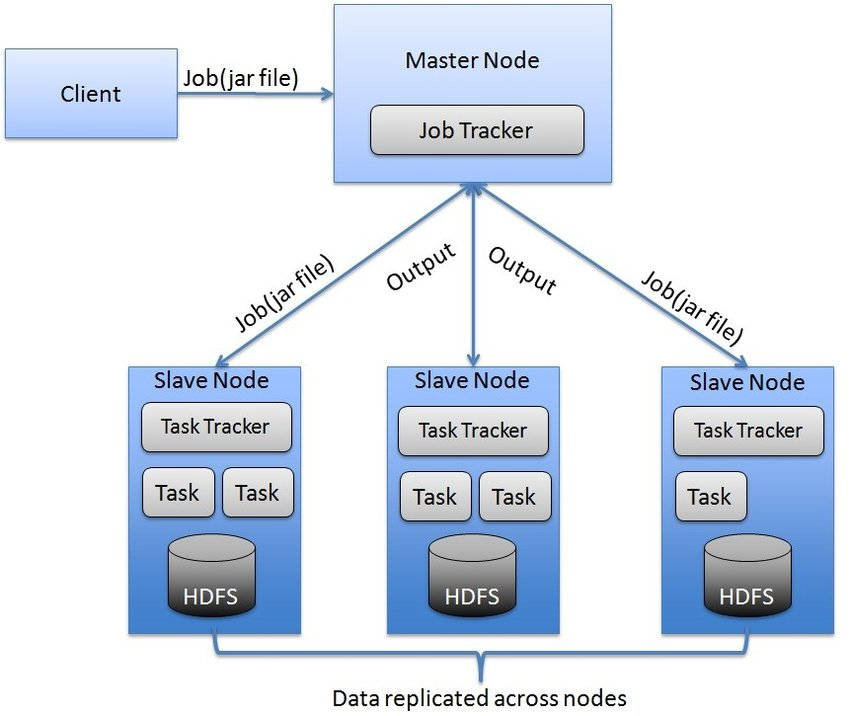
\includegraphics[scale=0.45]{document/chapters/chapter_4/images/hadoop_master_slave_architecture.png}
    \caption{Hadoop's MapReduce master-slave architecture\cite{hadoop_map_reduce}}
    \label{fig:hadoop_master_slave_architecture}
\end{figure}

A Client machine resides Outside the cluster and, when such machine needs to execute a MapReduce operation, firstly it needs to provide the Map and Reduce functions (written by the user that requests the task) to the Master (in Hadoop's case the code to execute is contained in a Jar file) which will propagate them to the Slaves. The Client also necessarily provides the data to process, whether sending them directly to the Master or specifying the source where to get them.

The Master machine has a Job Tracker through which it will coordinate the Slave machines; the worker machines, on the other hand, have a Task Tracker, through which information about the ongoing task can be accessed by the Master. Each Slave Node will have a queue of pending Tasks (sent by the Master) that will be executed and have access to the underlying Hadoop Distributed File System (HDFS) for data replication.